\section{Experimental Evaluation}

In this section we empirically analyze the performance of our classifiers. We employ the mean squared error (MSE) as the basic evaluation measure in our experiments, since we are primarily interested in evaluating sentiment scoring given by Equation~\ref{eq:prob}. The MSE measure is given as: 

\begin{equation}
\label{rmse}
\mathit{MSE} = \frac{1}{|\mathcal{T}|} \displaystyle\sum_{\forall t_i\in\mathcal{T}} (1 - \hat{p}(s_i|t_i))^2
\end{equation}
\noindent where $s_i$ is the correct sentiment associated with message $t_i\in\mathcal{T}$, and $\hat{p}(s_i|t_i)$ is the sentiment score assigned by the classifier to message $t_i\in\mathcal{T}$.

To evaluate the amount of computing resources used as the stream evolves, we employ the RAM-Hours measure~\cite{Bifet:2010:FPD:2144032.2144069}, where every RAM-Hour equals a GB of RAM deployed for 1 hour of execution. We also evaluate the amount of training resources used over time, as the number of messages labeled during the process. We used Hoeffding Adaptive Trees~\cite{bifetsent1,bifetsent2} (abbreviated as HAT), Active Classifier~\cite{6414645,Indre2011k} (abbreviated as AC), and Incremental Lazy Associative Classifier~\cite{sigir} (abbreviated as ILAC) as baselines. All datasets used in our experiments were manually labeled by three to five human annotators.
We expended significant time, effort,
and resources to obtain high quality (labeled) data from Twitter streams,
which shall be made available at publication time.

All experiments were performed on a 1.93 GHz Core i7 machines with 8GB of memory, using the MOA system \cite{moa}, an environment for running experiments with evolving data streams.
Our evaluation follows the Test-Then-Train methodology, in which 
each individual message in $\mathcal{T}$ is used to test the classifier
and then it becomes available for training.
Finally, we consider two possible settings: 
\begin{itemize}
\item{\bf{Instance Processing $-$}}
Once processed, message $t_n$ is included into $D_{n+1}$, and then a new classifier is built. Under this setting, message $t_n$ is mandatorily labeled.
\item{\bf{Batch Processing $-$}}
After a batch of $b$ messages $B=\{t_n,$ $t_{n+1},$ $\ldots, t_{n+b}\}$ is processed, only a subset of $B$ is included into $D_{n+b}$, since some messages in $B$ may be similar to each other. Under this setting, not all messages in $B$ need to be labeled, since only a subset of $B$ is included into $D_{n+b}$. Therefore, there is a trade-off between batch size and labeling effort, and a similarity threshold, denoted as $\alpha$, controls the messages in the batch that must be labeled.
\end{itemize}

In the following we describe our evaluation scenarios and discuss the
performance of the classifiers.

\subsection{Brazilian Presidential Elections}

The presidential election campaigns were held from June to October 2010.
the candidate Dilma Rousseff launched a Twitter page during a public announcement, and she used Twitter as one of the main sources of information for her voters. The campaign attracted more than 500,000 followers and
as a result Dilma was the second most cited person on Twitter in 2010.
The election came to a second round vote, and Dilma Rousseff won the runoff with 56\% of the votes.

\paragraph*{\bf{Dilma Rousseff Election Campaign}} We collected 66,643 messages in Portuguese referencing Dilma Rousseff in Twitter during her campaign. We labeled these messages in order to track the population sentiment of approval during this period. As shown in Figure~\ref{fig:dilma} (a), approval varied greatly over the time due to several polemic statements and political attacks, and our goal is to score approval during her campaign.
%The dataset contains 62,089 distinct terms, and
%a message is posted every 50 seconds, on average.

\begin{figure*}[htb]
\centering
\subfigure[Approval over Dilma Rousseff's campaign. Approval sentiment varied greatly from 05/2010 to 11/2010.]{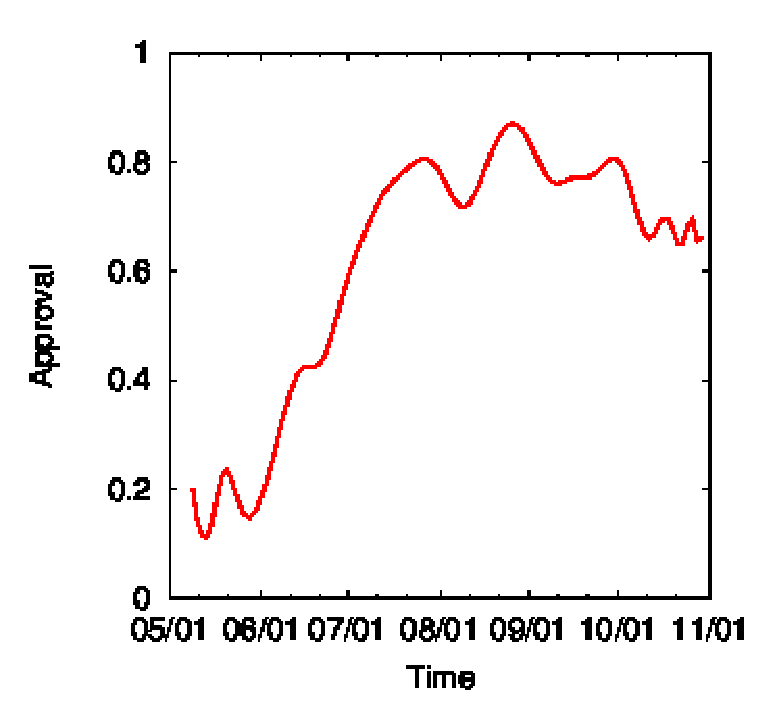
\includegraphics[width=2.1in,height=1.6in]{dilmaPositividade.eps}}
\subfigure[MSE numbers as the stream evo\-lves.]{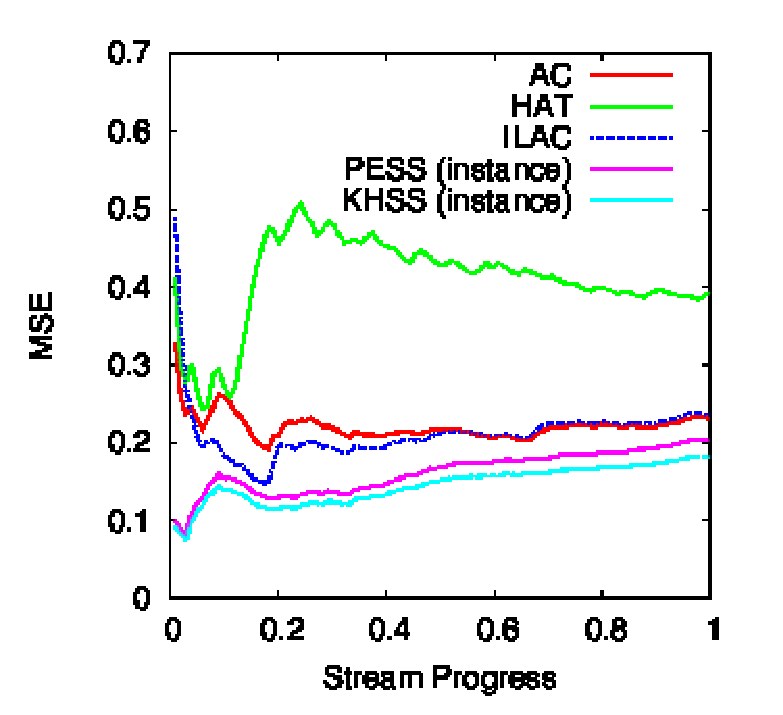
\includegraphics[width=2.1in,height=1.6in]{dilma_1_temporal_mse.eps}}
\subfigure[X-Y scatter plot correlating the minimum similarity threshold $\alpha$ and labeling effort.]{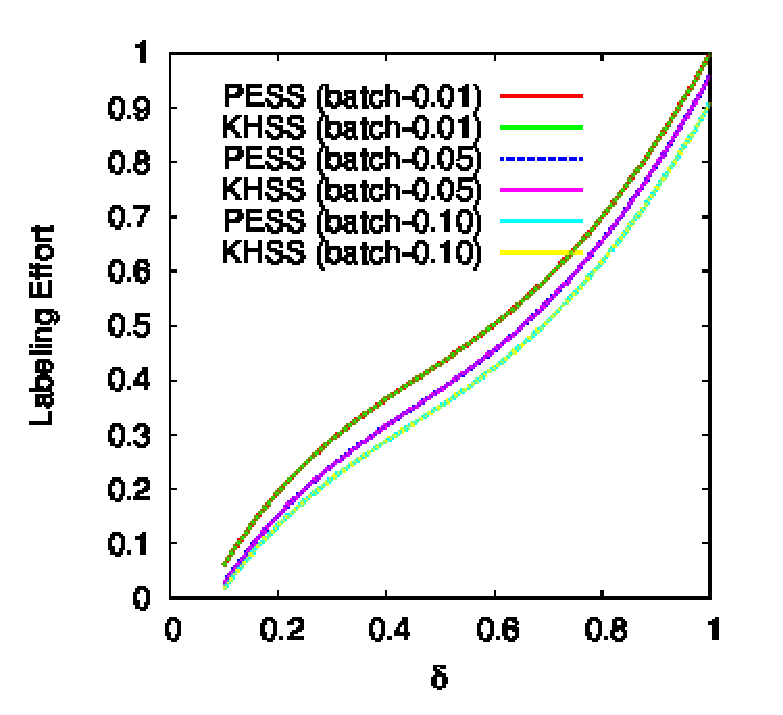
\includegraphics[width=2.1in,height=1.6in]{dilma_2_similaridade_rotulacoes.eps}}
\subfigure[X-Y scatter plot correlating labeling effort and MSE numbers.]{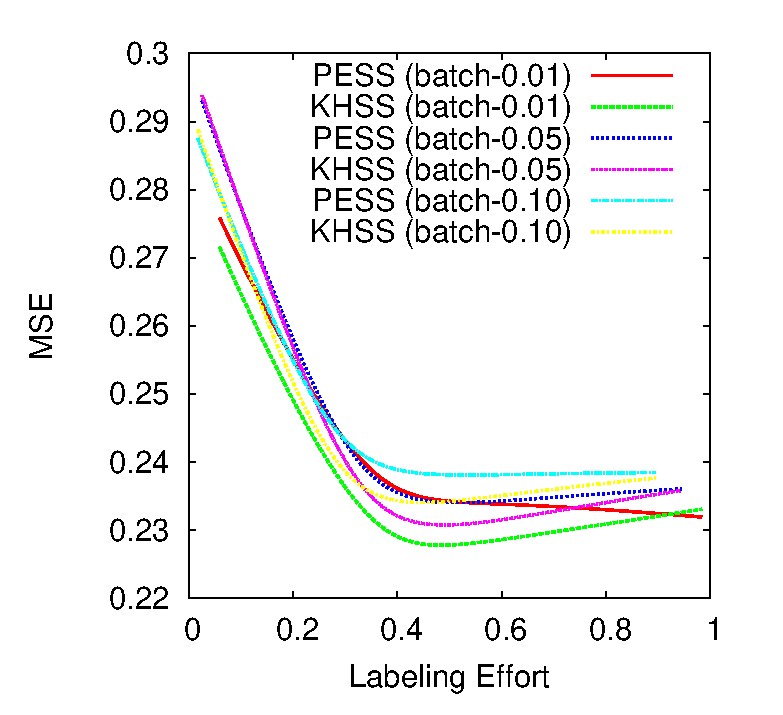
\includegraphics[width=2.1in,height=1.6in]{dilma_3_rmse-labelling.eps}}
\subfigure[Training windows as the stream evolves.]{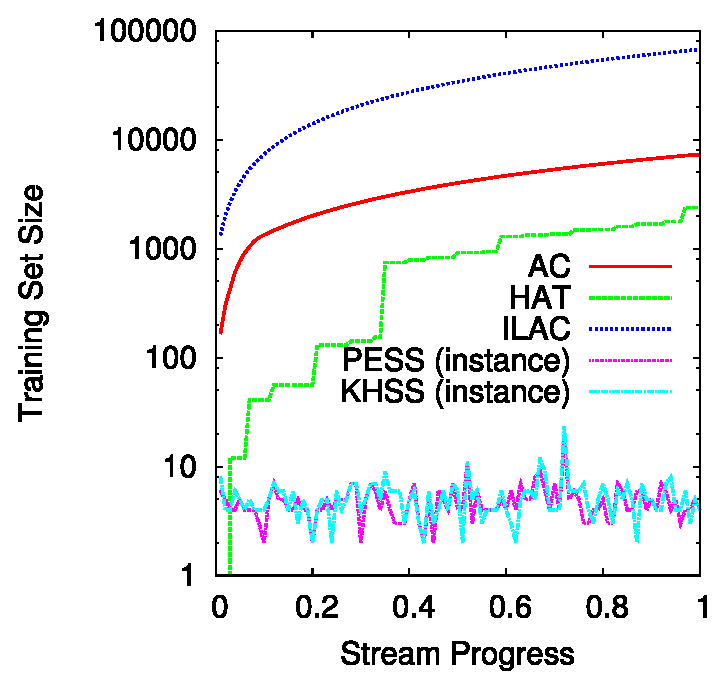
\includegraphics[width=2.1in,height=1.6in]{dilma_window.eps}}
\subfigure[RAM-Hours as the stream evo\-lves.]{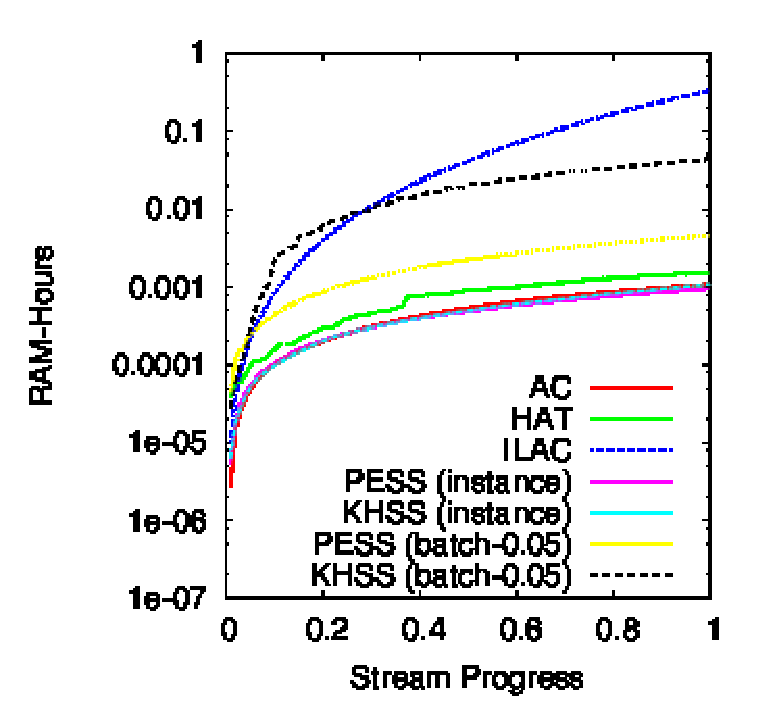
\includegraphics[width=2.1in,height=1.6in]{dilma_4.1_ram-hours_instance_baseline.eps}}
\caption{Brazilian Presidential Elections. Tweets are in Portuguese.}
\label{fig:dilma}
\end{figure*}

Figure~\ref{fig:dilma} (b) shows the results in terms of MSE obtained for the evaluation of the classifiers in this dataset. All classifiers evaluated in this experiment operate on an instance basis.
The x-axis represents different time steps (i.e., each message that
passes in the stream), while the y-axis shows the MSE so far.
As can be seen, a better approximation is obtained using our proposed algorithms, namely PESS and KHSS.
%For this dataset, HAT was not effective, as its performance deteriorates as the stream evolves.
AC and ILAC were very competitive during all the campaign. Both PESS and KHSS algorithms started much better than the other competing algorithms, but slowly converges to the baseline numbers as the stream evolves.

Figure~\ref{fig:dilma} (c) shows results concerning the proposed algorithms when operating in batch mode. The figure shows the number of messages that were labeled during the process as a function of $\alpha$, the minimum similarity threshold discussed in Section 3.1. Basically, we calculate the Jaccard coefficient associated with each possible pair of messages in the batch, and if the coefficient is greater than $\alpha$, the corresponding messages are merged into a new one. The process continues merging similar messages until no pair of messages are similar enough, and the process stops. At the end, only the merged messages are labeled. Clearly, higher values of $\alpha$ implies that less messages are merged, and thus incurring more labeling effort. Further, as the figure shows, the dependence between labeling effort and $\alpha$ tends to be linear.
%Also, both algorithms, PESS and KHSS, require the same amount of training resources during the process.

By varying $\alpha$, we also study the trade-off between labeling effort and MSE. As shown in Figure~\ref{fig:dilma} (d), MSE decreases if more labeling effort is spent during the process. Specifically, best results are achieved when about 40\% of the messages in the stream are labeled during the process. Although both PESS and KHSS require the same amount of training resources, KHSS provides slightly better MSE numbers. Furthermore, smaller batch sizes incur in less labeling effort for this dataset.

\begin{figure*}[htb]
\centering
\subfigure[MSE of different setups.]{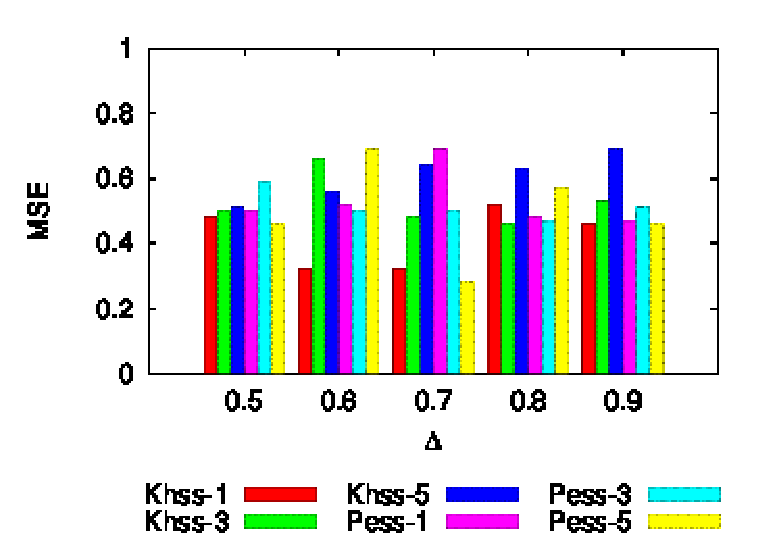
\includegraphics[width=2.1in,height=1.6in]{dilma_g-rmse.eps}}
\subfigure[Percentage of messages correctly included in the training set.]{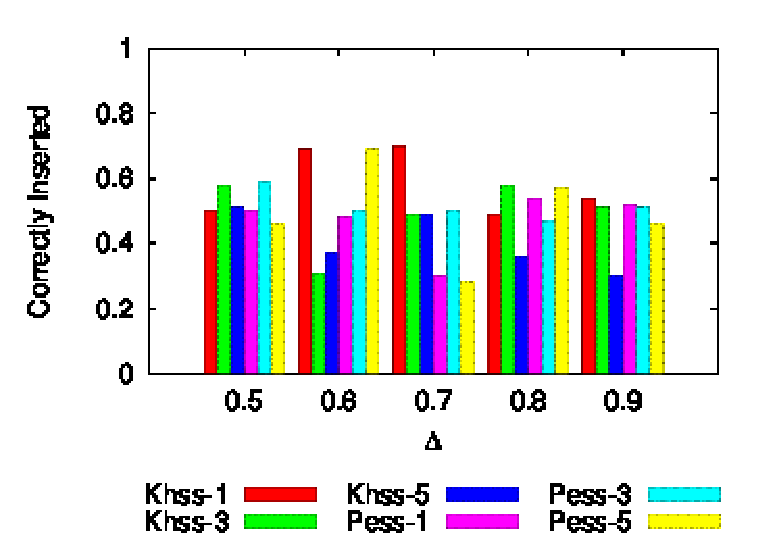
\includegraphics[width=2.1in,height=1.6in]{dilma_g-right.eps}}
\subfigure[MSE numbers as the stream evo\-lves.]{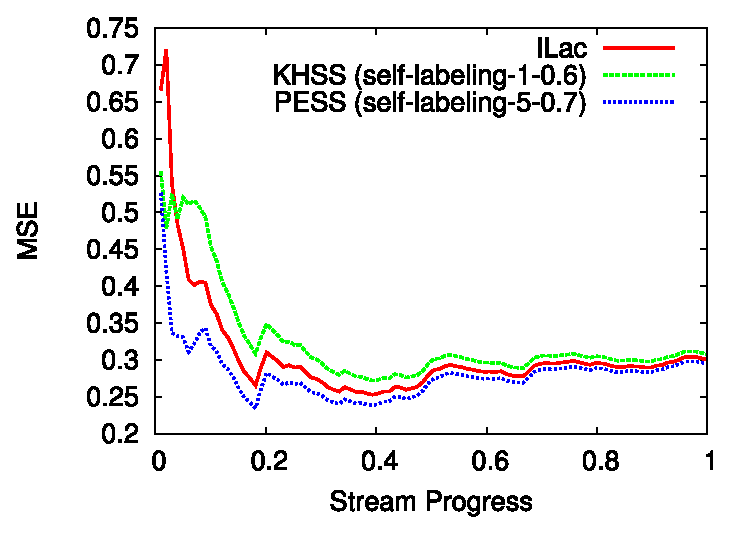
\includegraphics[width=2.1in,height=1.6in]{dilma_mse.eps}}
\subfigure[Training windows as the stream evolves.]{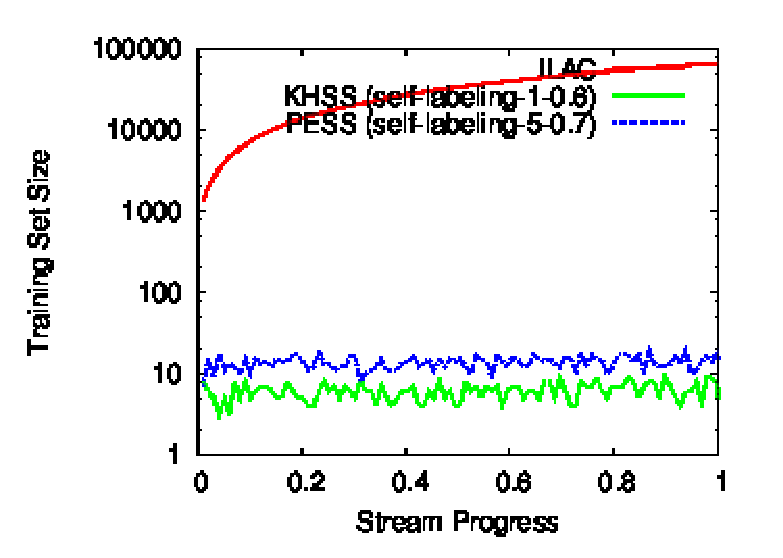
\includegraphics[width=2.1in,height=1.6in]{dilma_window_semi-super.eps}}
\subfigure[RAM-Hours as the stream evo\-lves.]{\includegraphics[width=2.1in,height=1.6in]{dilma_ramhours.eps}}
\caption{Brazilian Presidential Elections. Self-Labeling Algorithm.}
\label{fig:dilma-sl}
\end{figure*}

\begin{figure*}[htp]
\centering
\subfigure[MSE numbers as the stream evolves.]{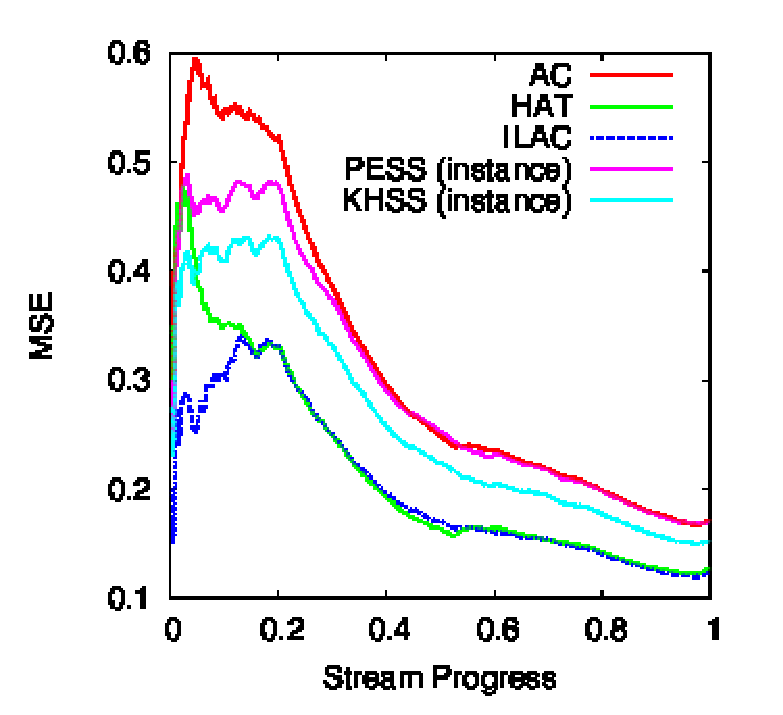
\includegraphics[width=2.1in,height=1.6in]{assange_1_temporal_mse.eps}}
\subfigure[X-Y scatter plot correlating labeling effort and MSE numbers.]{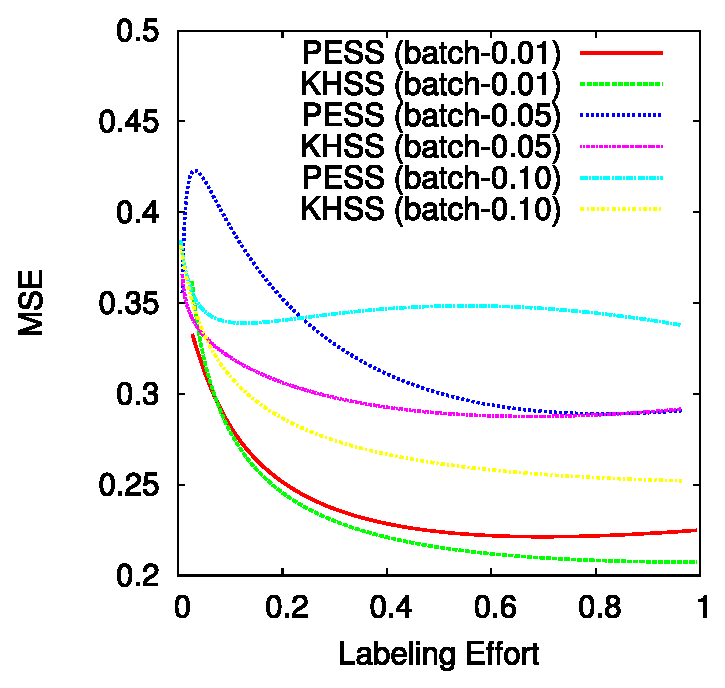
\includegraphics[width=2.1in,height=1.6in]{assange_3_rmse-labelling.eps}}
\subfigure[RAM-Hours as the stream evolves.]{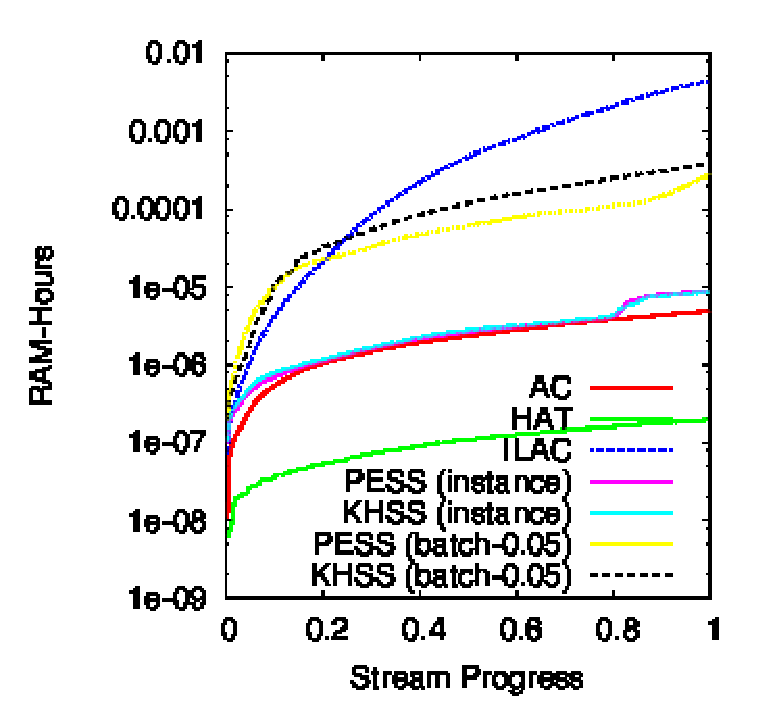
\includegraphics[width=2.1in,height=1.6in]{assange_4.1_ram-hours_instance_baseline.eps}}
\subfigure[Self-Labeling EESS algorithms. MSE numbers as the stream evo\-lves.]{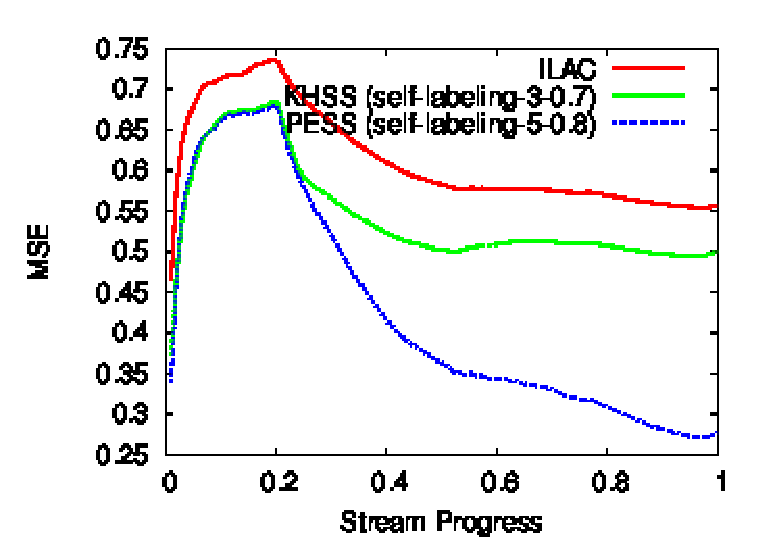
\includegraphics[width=2.1in,height=1.6in]{assange_mse.eps}}
\subfigure[Self-Labeling EESS algorithms. Training windows as the stream evolves.]{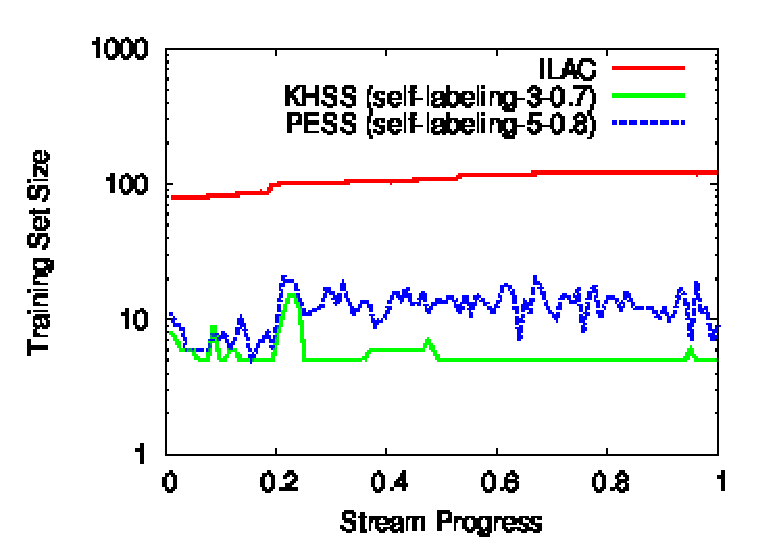
\includegraphics[width=2.1in,height=1.6in]{assange_window_semi-super.eps}}
\caption{Person of the Year. Tweets are in English.}
\label{fig:assange}
\end{figure*}

We assume that HAT requires only the target message for updating its tree model, and thus we consider that the training window is composed only by the target message. The AC algorithm requires much more
messages within each training window. An abrupt decrease in the number of training messages is always observed after drifts.
%Although ILAC performs a data projection strategy that filters irrelevant messages at each time step, it is clear that the number of training messages still increases as the stream evolves.
The proposed PESS algorithm requires very small training windows, since the Pareto frontier at each time step is composed by few messages, but these messages are still able to make the classifier robust to drifts as the stream evolves. Further, despite being less stringent than PESS, the proposed KHSS algorithm also requires small training windows, as shown in Figure~\ref{fig:dilma} (e).

Figure~\ref{fig:dilma} (f) shows RAM-Hours numbers for the algorithms. AC, as well as PESS (instance) and KHSS (instance), are clearly the best performers in terms of amount of computing resources required. Also, resources required during the process significantly increases when PESS and KHSS operate on batch mode, but still, ILAC is the worst performer.

Following in direction to reduction of labeling efforts we evaluate our Self-Labeling EESS algorithm. We choose as baseline ILAC algorithm with subjudice strategy. First we evaluate what setup achieved best results in terms of MSE. Figure~\ref{fig:dilma-sl} (a) shows that analysis. We also evaluate the correlation between MSE and amount of messages correctly labeled that were inserted in the training set. Figure~\ref{fig:dilma-sl} (b) shows that correlation and it is clear that the setup which label more accurately achieved lowest MSE as well. In Figure~\ref{fig:dilma-sl} (c) presents a comparison in terms of MSE over time between the best setup to PESS and KHSS against the baseline. PESS algorithms achieved lower MSE curve compared with ILAC. KHSS shown itself a close performance to ILAC. In terms of computational resources our both approaches were better than ILAC requiring less RAM-Hours(Figure~\ref{fig:dilma-sl} (d)). That can also be seen in Figure~\ref{fig:dilma-sl} (e) which show the amount of messages as the training set. Our approaches keep the training set as small as possible and up-to-date in relation to the current stream concept. 

\subsection{TIME's Person of the Year}

Every year, TIME magazine selects the person (or a group of persons) that
has mostly influenced during the year. The chosen person for 2010 was Mark Zuckerberg. The reader choice, however, was Julian Assange, with an overwhelming superiority of votes.

\paragraph*{\bf{Zuckerberg and Assange}}
We collected 5,616 messages in English
referencing Julian Assange and Mark Zuckerberg from 1-15-2010 to 12-21-2010.
We labeled them in order to track diverse sentiments regarding the magazine's decision. Sentiments include (dis)approval, surprise (since the reader choice was pointing to Julian Assange),
and even fury.
%The dataset contains 7,294 distinct terms, and
%a message is posted every 45 seconds, on average.

Figure~\ref{fig:assange} (a) shows the results in terms of MSE.
%The x-axis represents each message that
%passes in the stream, while the y-axis shows the MSE so far.
As can be seen, a better approximation is obtained by HAT and ILAC.
For this dataset, AC was not effective in the first
time steps. At the end of the process, both PESS (instance) and KHSS (instance) algorithms achieved competitive numbers when compared against the best performers.

Figure~\ref{fig:assange} (b) shows the trade-off between labeling effort and MSE. Again, MSE numbers decrease as more labeling effort is spent during the process. This trend is particularly evidenced for smaller batch sizes. Further, the KHSS algorithms shows a better compromise between labeling effort and MSE.
Figure~\ref{fig:assange} (c)
shows RAM-Hours numbers for the evaluated algorithms. The AC algorithm, as well as PESS (instance) and KHSS (instance) are, again, extremely competitive in terms of amount of computing resources required. Further, the amount of resources required during the process significantly increases when PESS and KHSS operate on batch mode, but still, ILAC is the worst performer.
Figure~\ref{fig:assange} (d) shows the results of our Self-Labeling EESS algorithms. As can be seen, both of our algorithms (PESS and KHSS) achieved better approximation where PESS was better than KHSS.
As shown in Figure~\ref{fig:assange} (c) ILAC require more computational resources than EESS algorithms. The same happens in the Self-Augmenting setup of ILAC due the amount of messages in the training set. Figure~\ref{fig:assange} (e) shows the number of messages required by EESS algorithms in contrast with ILAC. Our algorithms keep the training set as small as possible to be consistent with the current concept of the stream.


\subsection{FIFA World Cup}

The 2010 Soccer World Cup involved 32 teams. The Brazilian team was defeated by the Dutch team on 07-02-2010, after a controversial match. The Brazilian team scored first, but soon after the Dutch team scored twice and won the match. A specific player, Felipe Melo, had decisive participation (for better and worse) in all three goals. Specifically, Figure~\ref{fig:por} (a) shows how the appreciation for Felipe Melo varied during the match.

\paragraph*{{The Brazilian Defeat}} We collected 3,214 messages in Portuguese referencing Felipe Melo that were posted in Twitter as the match was happening.
We labeled them in order to track the
appreciation for the participation of Felipe Melo.

\begin{figure*}[htb]
\centering
\subfigure[Appreciation associated with Felipe Melo over the match.]{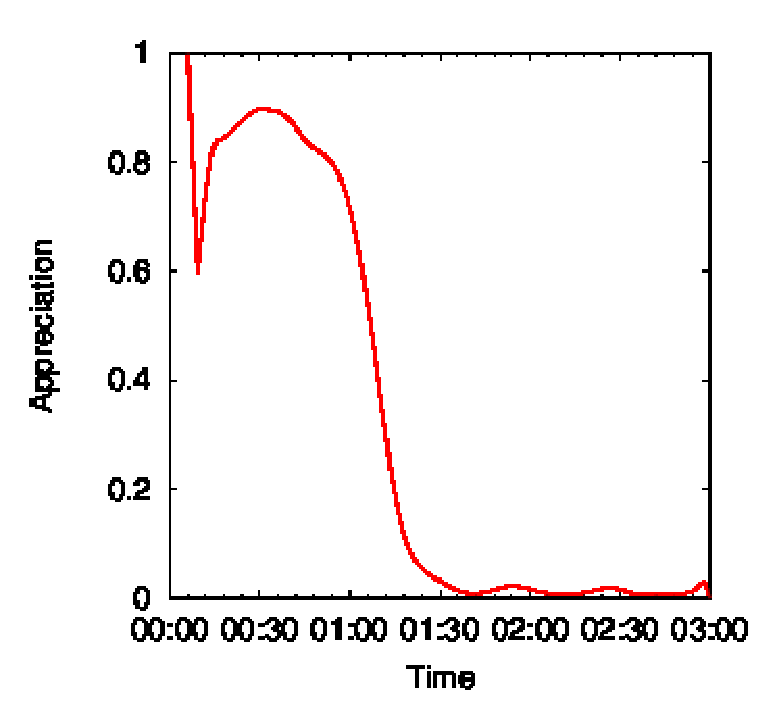
\includegraphics[width=2.1in,height=1.6in]{felipemeloPositividade.eps}}
\subfigure[MSE numbers as the stream evolves.]{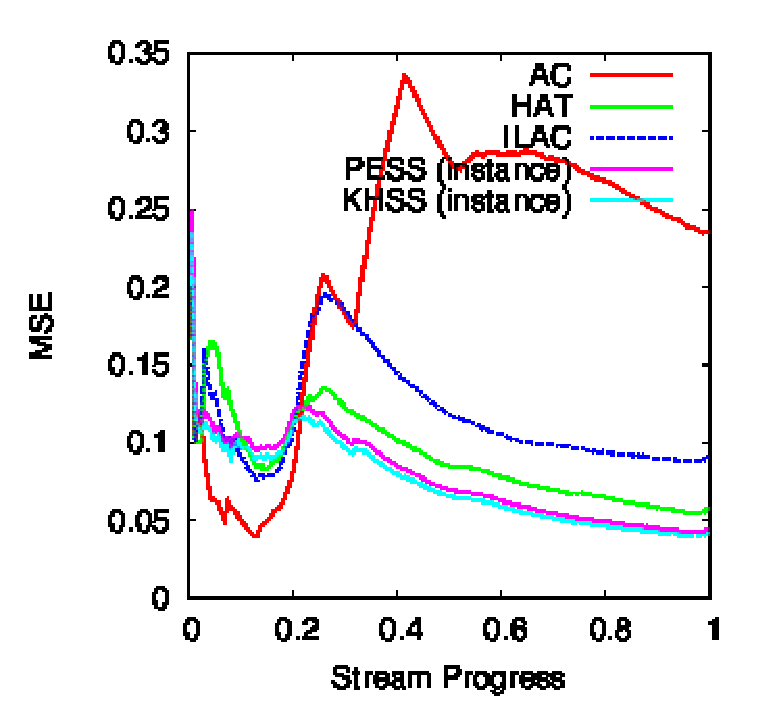
\includegraphics[width=2.1in,height=1.6in]{pt_1_temporal_mse.eps}}
\subfigure[X-Y scatter plot correlating the minimum similarity threshold $\alpha$ and labeling effort.]{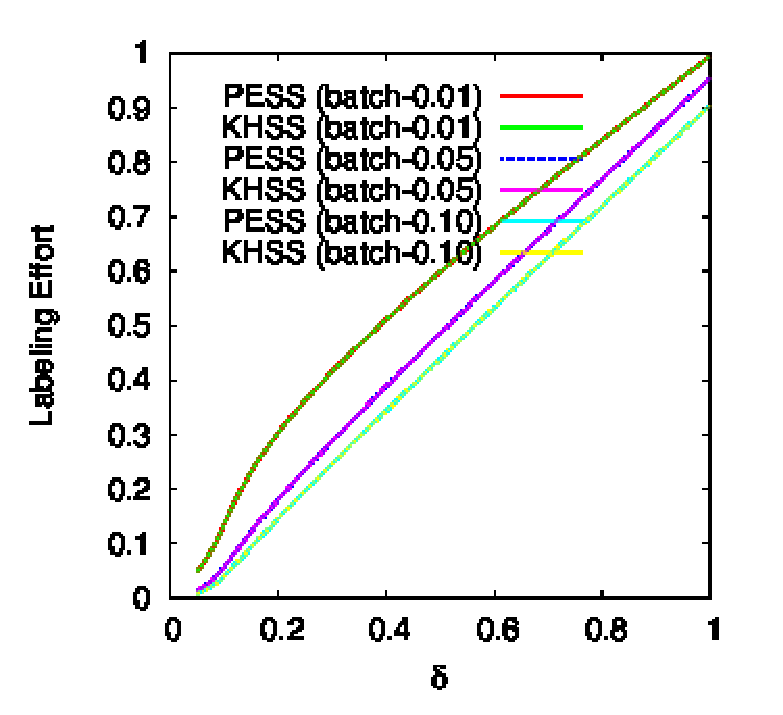
\includegraphics[width=2.1in,height=1.6in]{pt_2_similaridade_rotulacoes.eps}}
\subfigure[X-Y scatter plot correlating labeling effort and MSE numbers.]{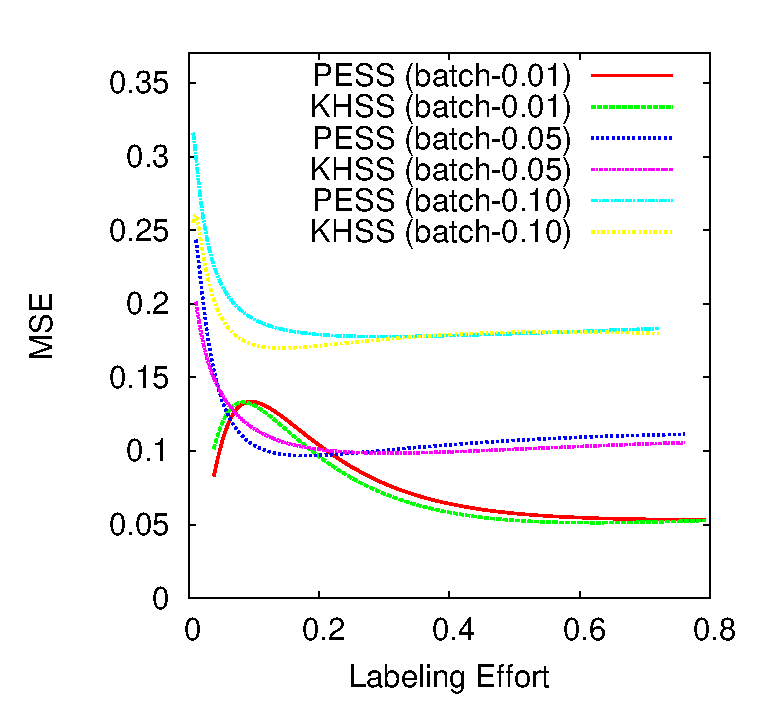
\includegraphics[width=2.1in,height=1.6in]{pt_3_rmse-labelling.eps}}
\subfigure[Training windows as the stream evolves.]{\includegraphics[width=2.1in,height=1.6in]{pt_window.eps}}
\subfigure[RAM-Hours as the stream evolves.]{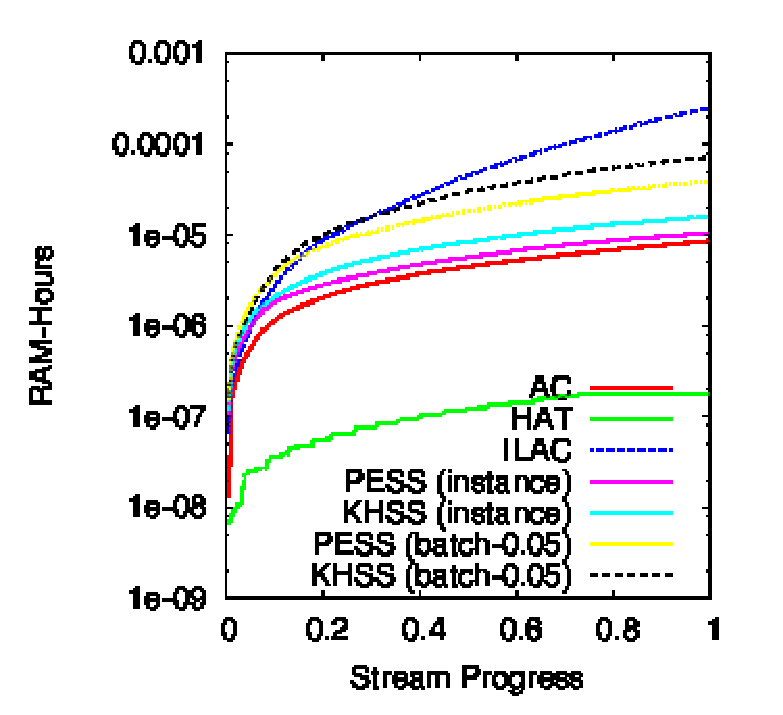
\includegraphics[width=2.1in,height=1.6in]{pt_4.1_ram-hours_instance_baseline.eps}}
\caption{The Brazilian Defeat. Tweets are in Portuguese.}
\label{fig:por}
\end{figure*}

Figure~\ref{fig:por} (b) shows the results in terms of MSE.% We assume that these messages expose the sentiment expressed by Brazilian Twitter users during the match.
%Again, the x-axis represents each message that
%passes in the stream, while the y-axis shows the MSE so far.
As can be seen, the AC algorithm achieved the worst MSE numbers for this dataset. On the other hand, HAT, ILAC, as well as PESS (instance) and KHSS (instance) showed extremely competitive numbers. This is expected, since this dataset contains three sudden drifts (as shown in Figure~\ref{fig:por} (a)), and HAT, ILAC, PESS (instance) and KHSS (instance) were all able to ensure adaptiveness.
%either by updating the tree model or projecting the training window according to the target message, or by selecting messages by minimizing time and space distances.
For this dataset, memorability is not mandatory (as the sentiment distribution never returns to a pre-drift
distribution), and thus PESS (instance) and KHSS (instance) were not able to provide significant improvements, although being the best performers overall.

Figure~\ref{fig:por} (c) shows a X-Y scatter plot correlating $\alpha$ and labeling effort. The correlation is almost linear. The trade-off between labeling effort and MSE is shown in Figure~\ref{fig:por} (d). Clearly, MSE decreases with the effort spent to label messages.
Figure~\ref{fig:por} (e) shows the number of messages composing the training window at each time step.
As in previous cases, AC and ILAC require much more training resources than other competing algorithms. PESS (instance) as well as KHSS (instance) require much less training messages, again, showing that the selective sampling strategy is effective in producing small and effective windows at each time step.

Figure~\ref{fig:por} (f)
shows RAM-Hours numbers. In this case, AC, as well as PESS (instance) and KHSS (instance), are clearly the best performers in terms of amount of computing resources required. Further, the amount of resources required during the process significantly increases when PESS and KHSS operate on batch mode, but still, as in other datasets, ILAC is the worst performer.

\begin{figure*}[htb]
\centering
\subfigure[MSE of different setups.]{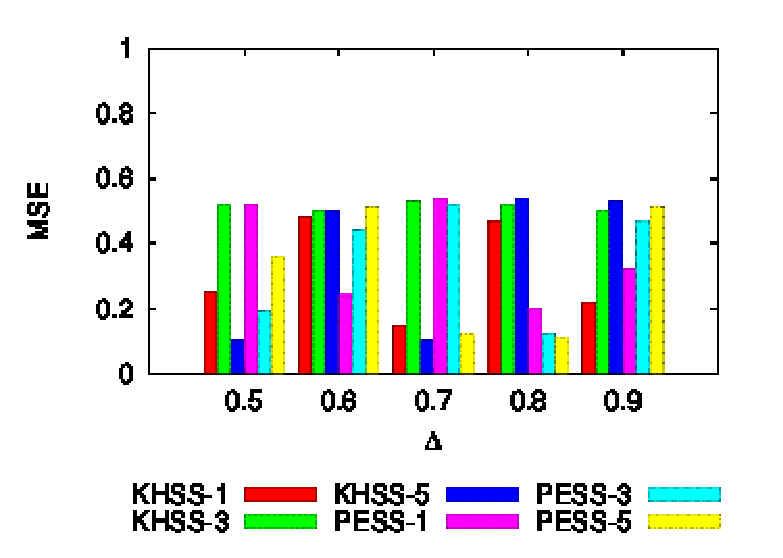
\includegraphics[width=2.1in,height=1.6in]{pt_g-rmse.eps}}
\subfigure[Percentage of messages correctly included in the training set.]{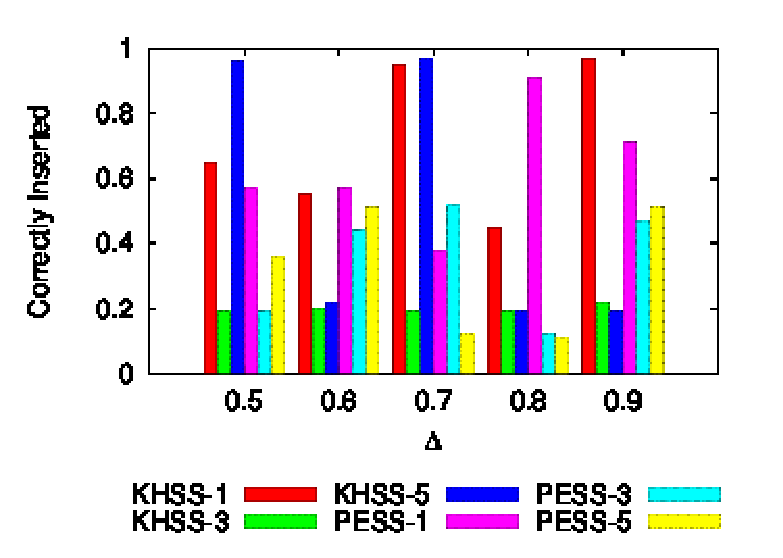
\includegraphics[width=2.1in,height=1.6in]{pt_g-right.eps}}
\subfigure[MSE numbers as the stream evo\-lves.]{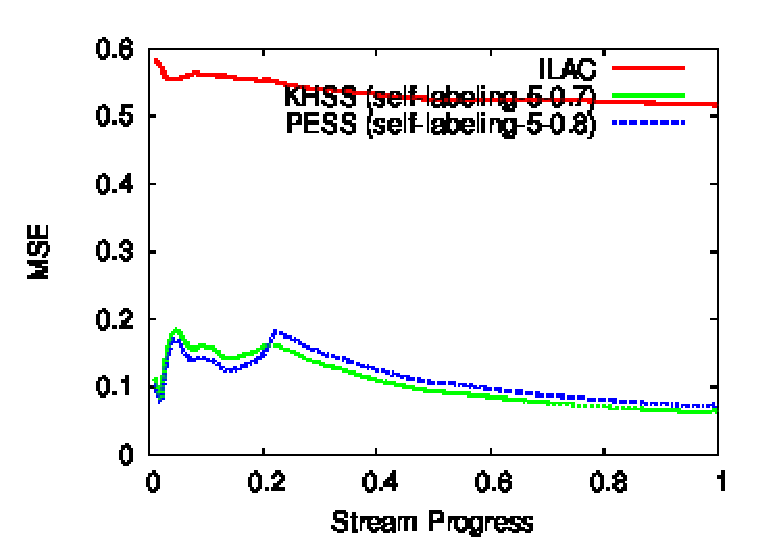
\includegraphics[width=2.1in,height=1.6in]{pt_mse.eps}}
\subfigure[RAM-Hours as the stream evo\-lves.]{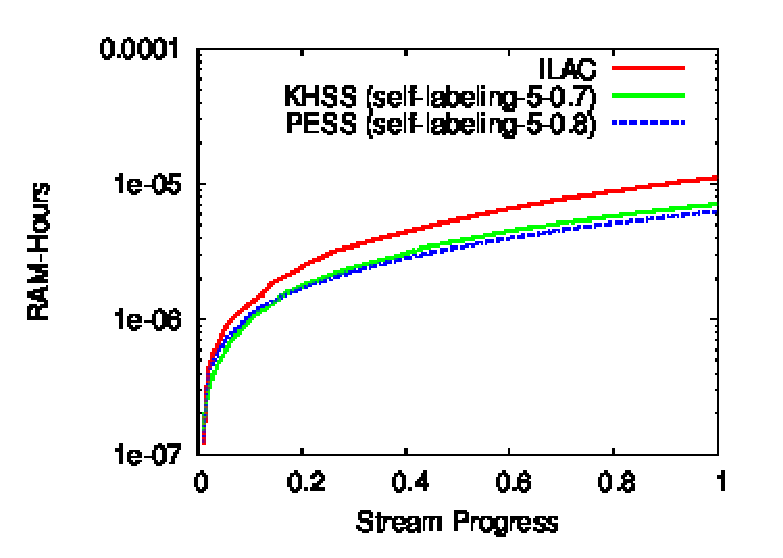
\includegraphics[width=2.1in,height=1.6in]{pt_ramhours.eps}}
\caption{The Brazilian Defeat. Self-Labeling Algorithm.}
\label{fig:por-sl}
\end{figure*}

We evaluate our Self-Labeling EESS algorithms in this dataset in order to select the best setup. Figure~\ref{fig:por-sl} (a) shows the MSE of several setups. As can be seen the setups which achieved better performance were PESS with 5 Independent Dimensions and Confidence Threshold 0.8 and KHSS with 1 Independent Dimension and Confidence Threshold 0.5. Figure~\ref{fig:por-sl} (b) shows that the best setups also included more accurately messages into training set. Figure~\ref{fig:por-sl} (c) shows the sentiment error approximation of ILAC and our EESS algorithms. As can be seen, our both algorithms are superior to ILAC providing better approximation. Further sentiment error approximation in evaluate the computational resources requires as well. Figure~\ref{fig:por-sl} (d) shows the RAM-Hours ratios of each algorithm. EESS algorithms need less computational resources than ILAC as can be seen.

%The last set of experiments concerns the evaluation of the same event, but using the dataset composed of messages in English. By inspecting the dataset, we confirmed that most of the messages were posted by people in Europe, specially German, English and Dutch users. Such users showed conflicting or mixed sentiments as the match goes. As a consequence, drifts occur, but eventually the sentiment distribution returns to a pre-drift distribution, making memorability an important property while scoring sentiments in this dataset. This explains the reason why PESS (instance) and KHSS (instance) performed much better than the other competitors, as we can see in Figure~\ref{fig:eng} (a). Figure~\ref{fig:eng} (b) shows the trade-off between MSE and the amount of training resources needed during the process. Finally, Figure~\ref{fig:eng} (c) shows the amount of computing resources needed during the process.

%\begin{figure*}[htb]
%\centering
%\subfigure[MSE numbers as the stream evolves.]{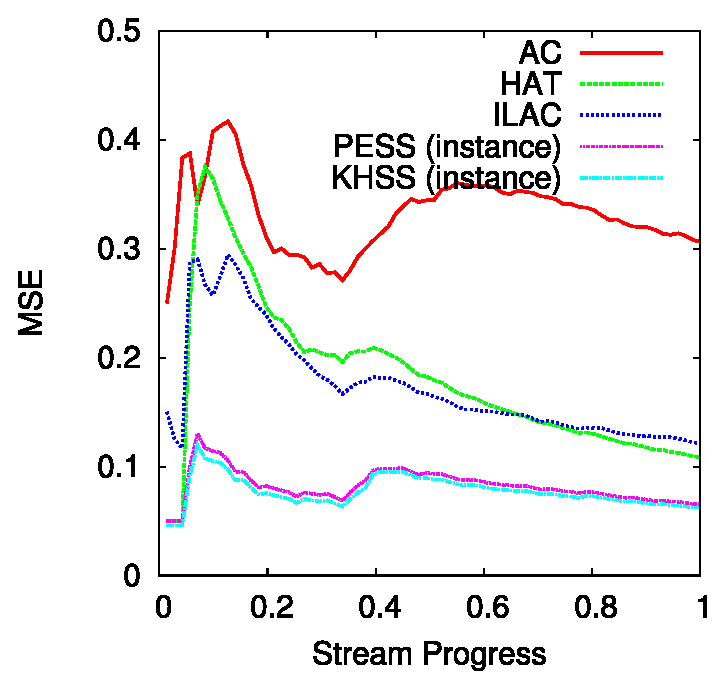
\includegraphics[width=2.1in,height=1.6in]{en_1_temporal_mse.eps}}
%\subfigure[X-Y scatter plot correlating labeling effort and MSE numbers.]{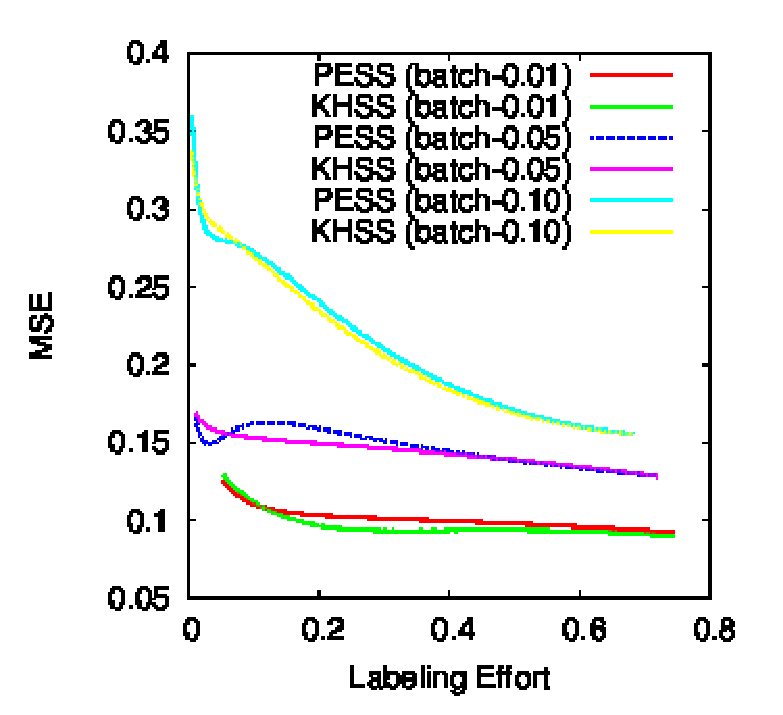
\includegraphics[width=2.1in,height=1.6in]{en_3_rmse-labelling.eps}}
%\subfigure[RAM-Hours as the stream evolves.]{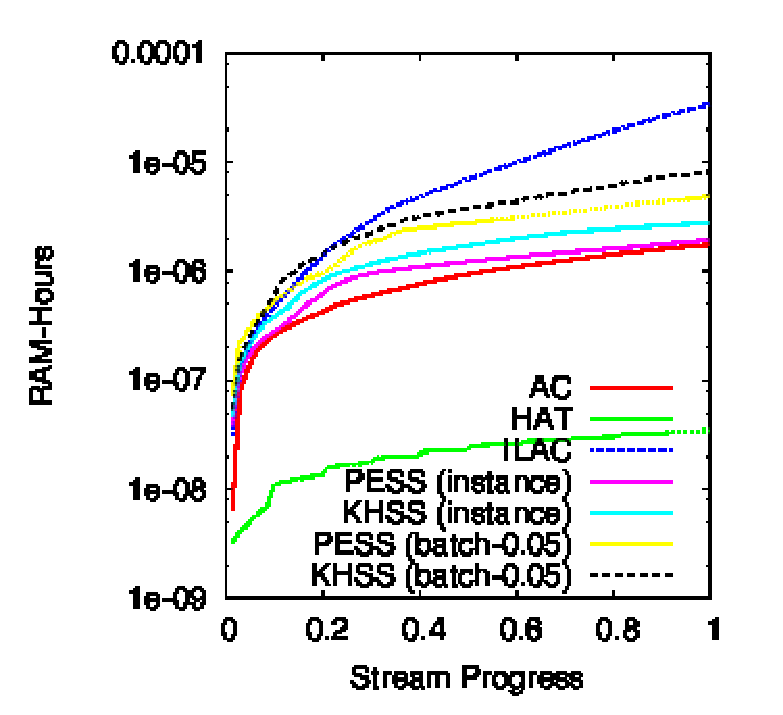
\includegraphics[width=2.1in,height=1.6in]{en_4.1_ram-hours_instance_baseline.eps}}
%\caption{The Brazilian Defeat. Tweets are in English.}
%\label{fig:eng}
%\end{figure*}
